\begin{mainquestion}{wye_delta_nodal}{Nodal Analysis + Delta/Wye}
Consider the following circuit. Note the top three resistors form a wye resistor network.

\begin{center}
    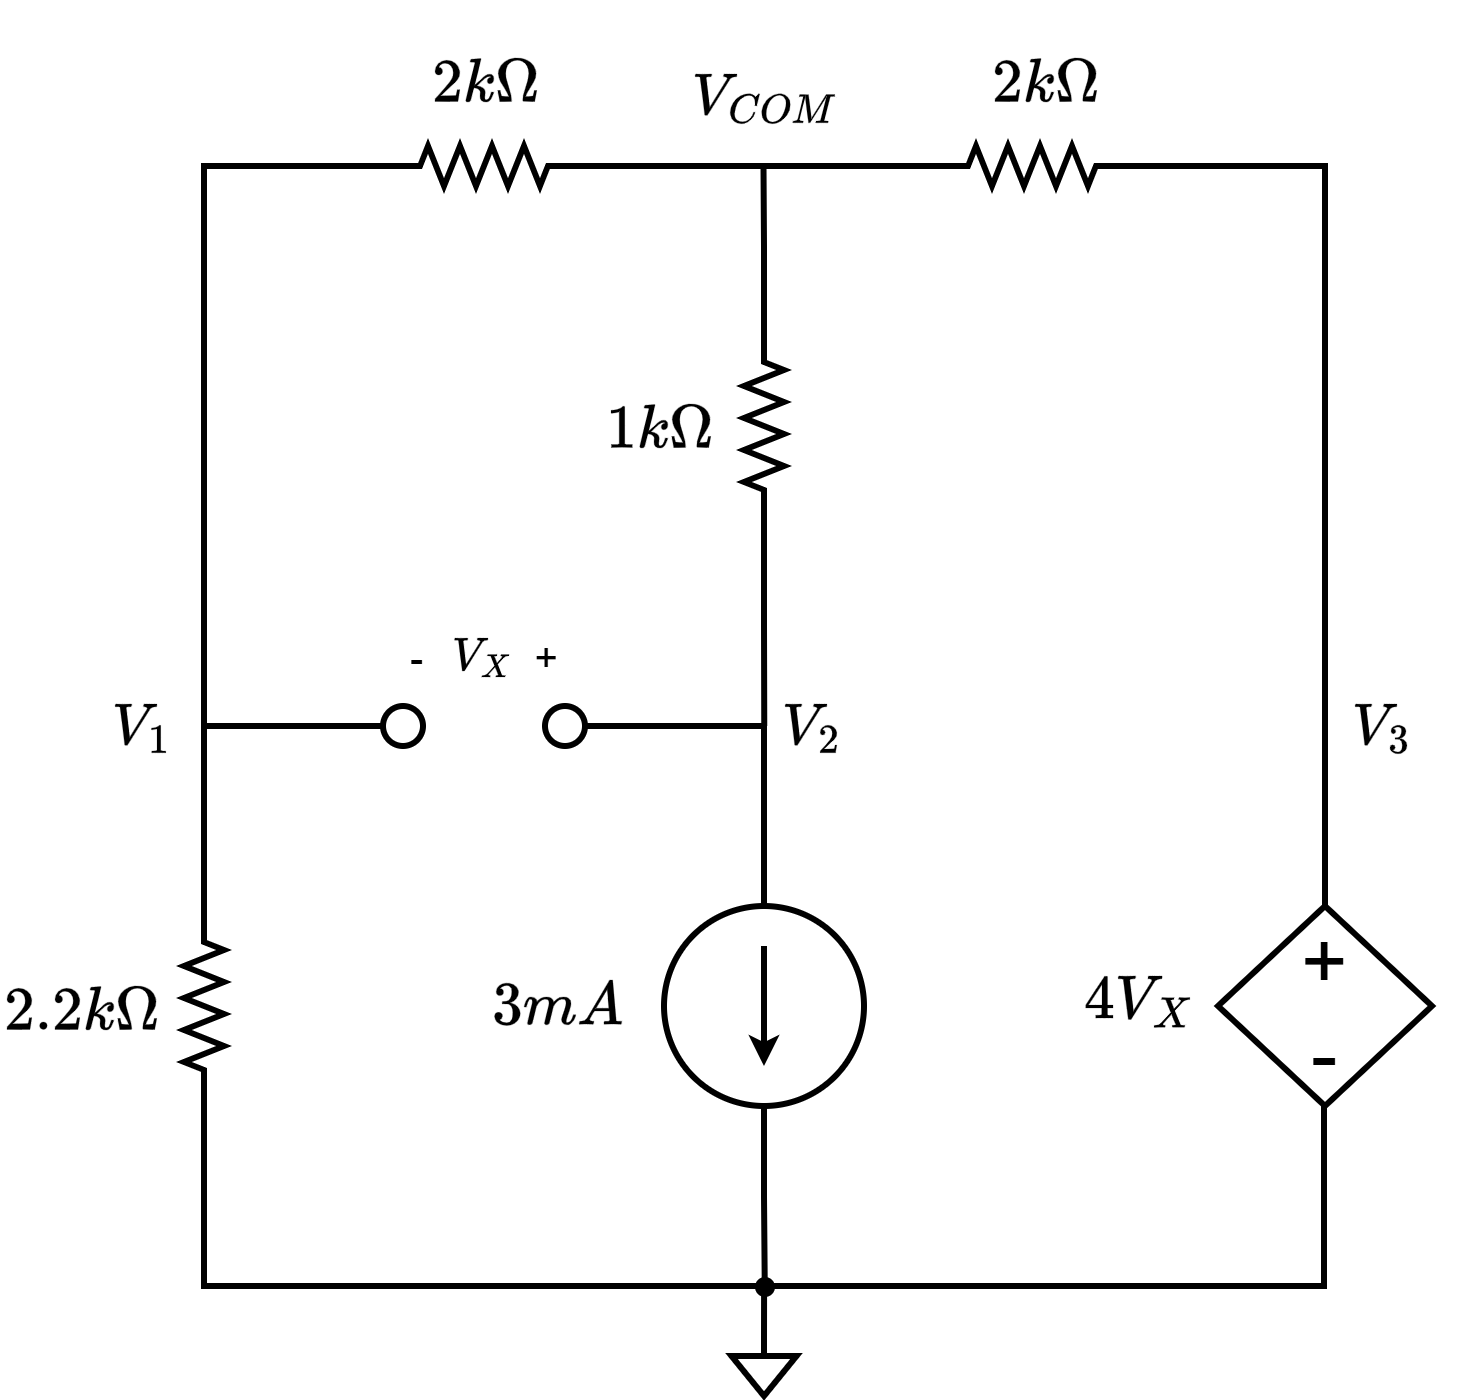
\includegraphics[width=0.6\textwidth]{questionbank/networks/wye_delta_nodal/v0/wye_sch.png}
\end{center}

% =========================================================
\begin{partquestion}{delta}
{Convert the wye network to a delta network with a Wye-Delta transform and redraw
the schematic. How many nodes exist in this equivalent circuit? How many nodes were
in the original?}
\begin{answer}
Looking at the Wye $\rightarrow$ Delta formulas, all of them use the same sum of the product pairs in their numerators. Let’s calculate that figure and we’ll call it $R_T$.
\[R_T=\ R_1R_2+R_2R_3+R_3R_1=4+2+2=\qty{8}{\mega\ohm}\]
Now we can calculate all the individual resistors. For the resistance between nodes $V_1$ and $V_2$, the equation will be $R_T/\qty{2}{\kilo\ohm} = \qty{4}{\kilo\ohm}$. For $V_2$ and $V_3$ we also have $R_T/\qty{2}{\kilo\ohm} = \qty{4}{\kilo\ohm}$ the odd one out will be the resistance between $V_1$ and $V_3$ which will be $R_T/\qty{1}{\kilo\ohm} = \qty{8}{\kilo\ohm}$. Here is the schematic with the new resistance values:

\begin{center}
    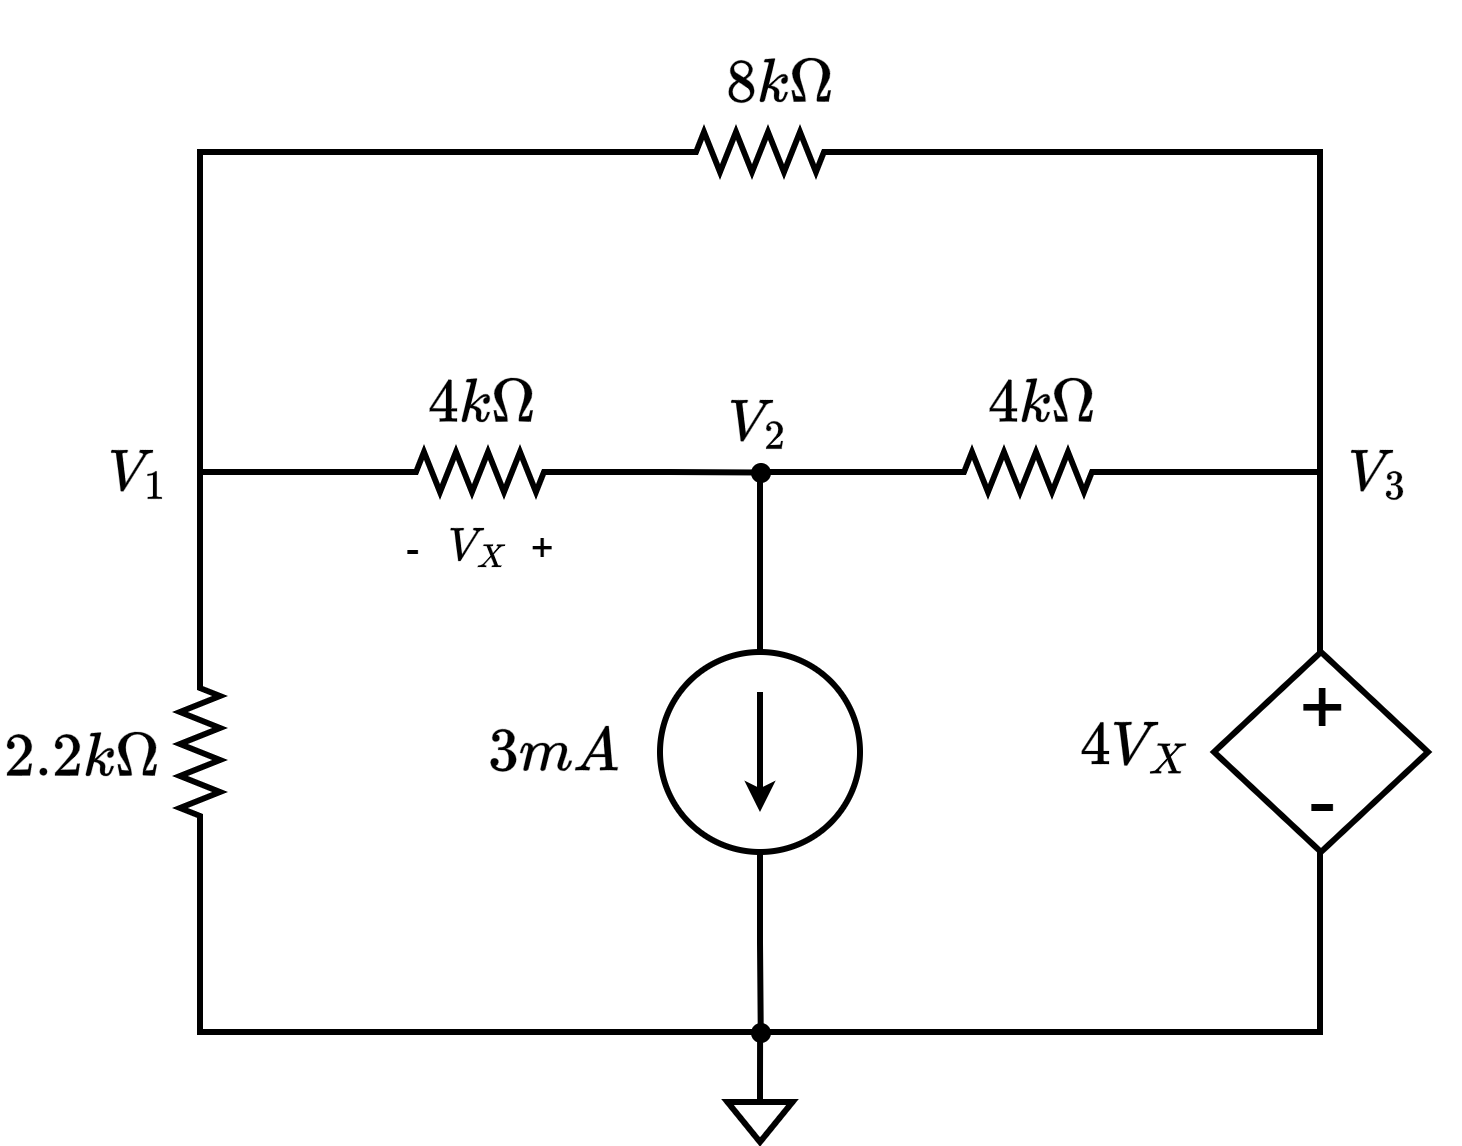
\includegraphics[width=0.5\textwidth]{questionbank/networks/wye_delta_nodal/v0/delta_sch_sol.png}
\end{center}

This new schematic has 4 nodes total, with only 3 independent nodes that require KCL equations. The original schematic had 5 nodes, with 4 independent nodes that need KCL equations. The transform effectively dropped one node for us.

\end{answer}
\end{partquestion}

% =========================================================
\begin{partquestion}{solve}
{Use nodal analysis on your new schematic to find each of the node voltages $V_1$, $V_2$ and $V_3$.}
\begin{answer}
We can leave out units, assuming all currents are \si{\milli\ampere}, all resistances are \si{\kilo\ohm}, and all voltages are \si{\volt}. Writing KCL using the nodal voltages at node 1 gives:
\begin{align*}
\frac{V_1}{2.2}+\frac{V_1-V_2}{4}+\frac{V_1-V_3}{8}&=0 \\
\frac{5V_1}{11}+\frac{V_1-V_2}{4}+\frac{V_1-V_3}{8}&=0 \\
40V_1+22(V_1-V_2)+11(V_1-V_3)&=0 \\
73V_1-22V_2-11V_3&=0
\end{align*}

Writing KCL using the nodal voltages at node 2 gives:
\begin{align*}
\frac{V_2-V_1}{4}+\frac{V_2-V_3}{4}+3&=0 \\
2V_2 - V_1 - V_3 &= -12
\end{align*}

We can see that $V_3 = 4V_x = 4(V_2 - V_1)$, so we can substitute this value into the two KCL equations above to get:
\begin{align*}
73V_1 - 22V_2 - 11\cdot 4(V_2 - V_1)&=0 \\
117V_1 - 66V_2 &= 0
\end{align*}
and
\begin{align*}
2V_2 - V_1 - 4(V_2 - V_1) &= -12 \\
-2V_2 + 3V_1 &= -12
\end{align*}

This gives two equations and two unknowns. Using your favorite method to solve systems of equations, we multiply the second equation by -33 and add the equations together to solve for the voltage at node 1:
\begin{align*}
117V_1 - 66V_2 - 33(-2V_2 + 3V_1) &= -33(-12) \\
18V_1 &= 396 \\
V_1 &= \qty{22}{\volt}
\end{align*}

Next we use this result with equation 2 to solve for the voltage at node 2:
\begin{align*}
-2V_2 + 3(22) &= -12 \\
V_2 &= \frac{-12 - 66}{-2} = \qty{39}{\volt}
\end{align*}

Now we can use \(V_1\) and \(V_2\) to solve for \(V_3\):

\[
V_3 = 4V_x = 4(V_2 - V_1) = 4(39 - 22) = \qty{68}{\volt}
\]
\end{answer}
\end{partquestion}

% =========================================================
\begin{partquestion}{findvx}
{Find $V_X$.}
\begin{answer}
\[V_X=V_2-V_1=39-22=\qty{17}{V}\]
Gotcha :)
\end{answer}
\end{partquestion}

% =========================================================
\begin{partquestion}{deltakcl}
{Given your results for $V_1$, $V_2$ and $V_3$, calculate all the branch currents in your new schematic. Show KCL is satisfied at each node.}

\begin{answer}
\begin{center}
    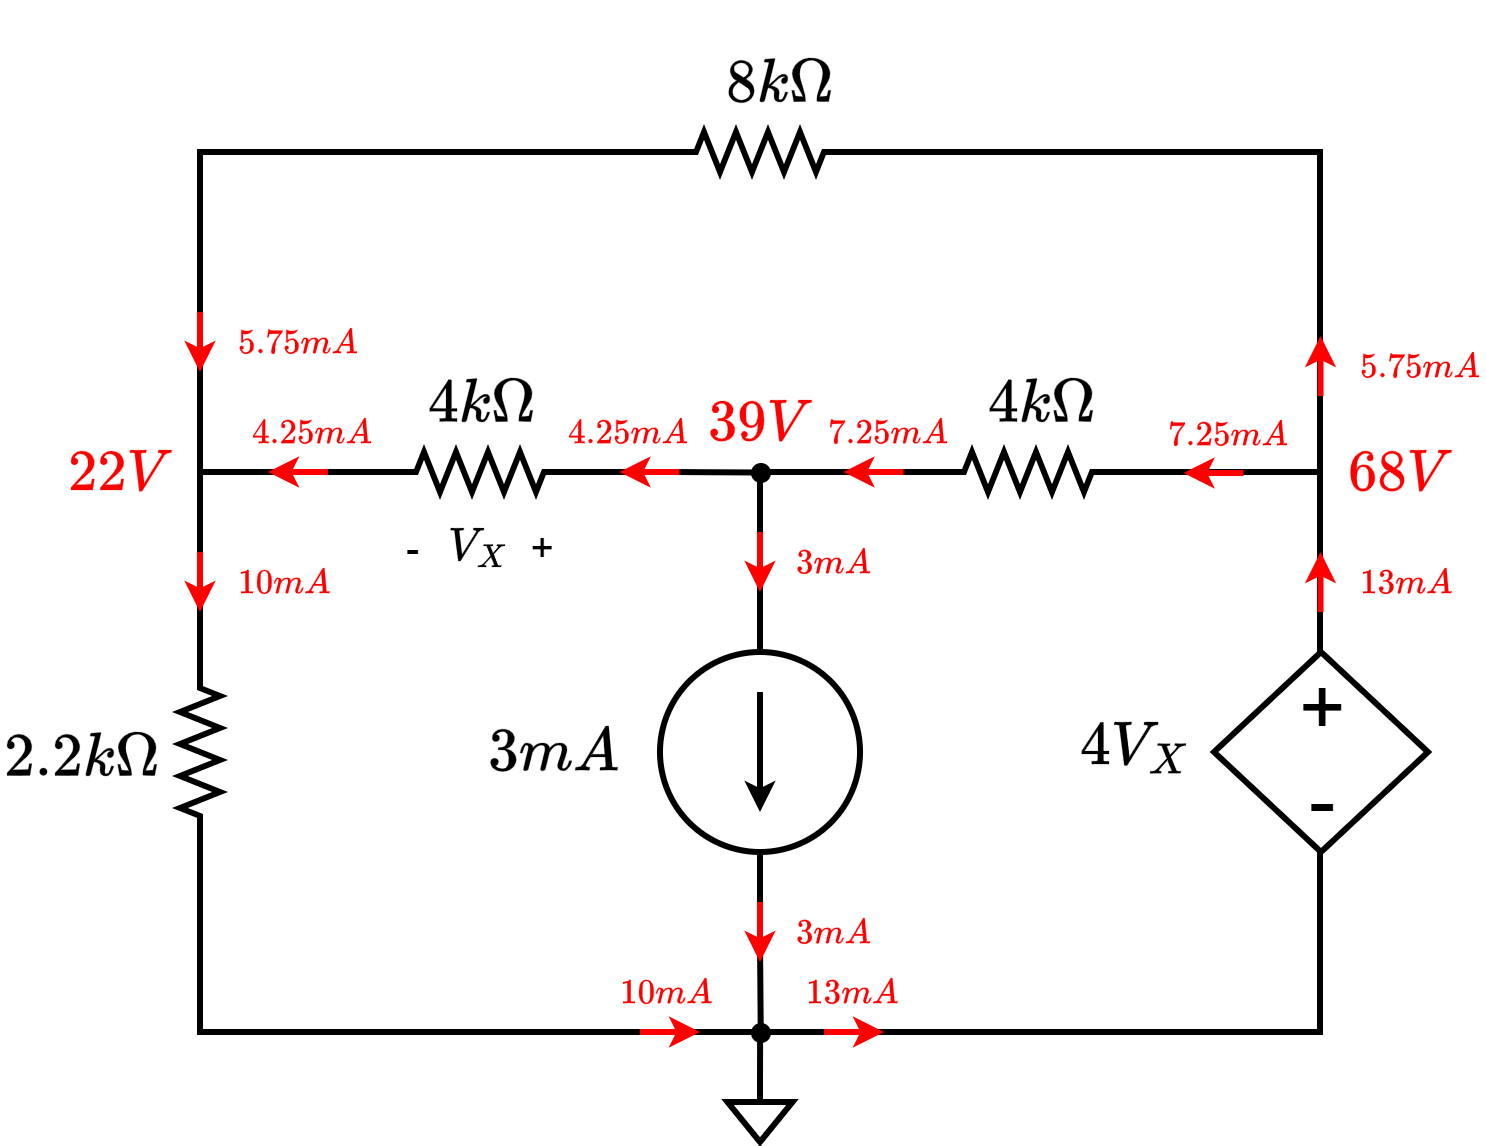
\includegraphics[width=0.5\textwidth]{questionbank/networks/wye_delta_nodal/v0/delta_kcl_sol.png}
\end{center}

Calculating the branch currents only requires Ohm’s Law for most of the branches. For example, the current through the top \qty{8}{\kilo\ohm} resistor is
\( I = \frac{V}{R} = \frac{\qty{68}{\volt} - \qty{22}{\volt}}{\qty{8}{\kilo\ohm}} = \qty{5.75}{\milli\ampere} \) and the current through the rightmost \qty{4}{\kilo\ohm} resistor is \( I = \frac{V}{R} = \frac{\qty{68}{\volt} - \qty{39}{\volt}}{\qty{4}{\kilo\ohm}} = \qty{7.25}{\milli\ampere} \). In a resistor, passive sign convention tells us that positive current flows in the direction of the voltage drop, so from left to right in this case. This can be repeated for the other resistors quite easily now that we have all of the voltage values. The only current that requires additional thought is the current through the dependent current source, which can be solved from the KCL equation at node 3.

\[
I_{4V_X} = I_{8k\Omega} + I_{4k\Omega} = \qty{5.75}{\milli\ampere} + \qty{7.25}{\milli\ampere} = \qty{13}{\milli\ampere}
\]

Now we check that KCL is satisfied everywhere. There are 4 nodes where KCL needs to hold in this schematic. We’ll use positive values for currents flowing into a node:

At Node 1: \( 5.75 + 4.25 - 10 = 0 \)

At Node 2: \( 7.25 - 4.25 - 3 = 0 \)

At Node 3: \( 13 - 5.75 - 7.25 = 0 \)

At Ground: \( 10 + 3 - 13 = 0 \)

Look at that! All copacetic. We are now confident our solution is correct.

\end{answer}
\end{partquestion}

% =========================================================
\begin{partquestion}{vcom}
{Returning to the original schematic, find the voltage $V_{\text{COM}}$ given your results for $V_1$, $V_2$ and $V_3$.}
\begin{answer}
This is not too hard since we know the current in the \qty{1}{\kilo\ohm} resistor because it’s in series with the \qty{3}{\milli\ampere} current source. Thanks to Ohm’s Law, we know that there must be a \qty{3}{\volt} drop across it. Passive sign convention tells us that the voltage is highest on the side the current is coming from, so that implies that $V_{\mathrm{COM}}$ is \qty{3}{\volt} higher than $V_2$.

\[
V_{\mathrm{COM}} = V_2 + 3 = 39 + 3 = \qty{42}{\volt}
\]

This could also be solved with similar math using the right (\qty{13}{\milli\ampere}) or left (\qty{10}{\milli\ampere}) branches, as we already know that currents flowing through them from part (\cref{prob:wye_delta_nodal:deltakcl}).

\end{answer}
\end{partquestion}

% =========================================================
\begin{partquestion}{wyekcl}
{Repeat part (\cref{prob:wye_delta_nodal:deltakcl}) for the original schematic.}
\begin{answer}
\begin{center}
    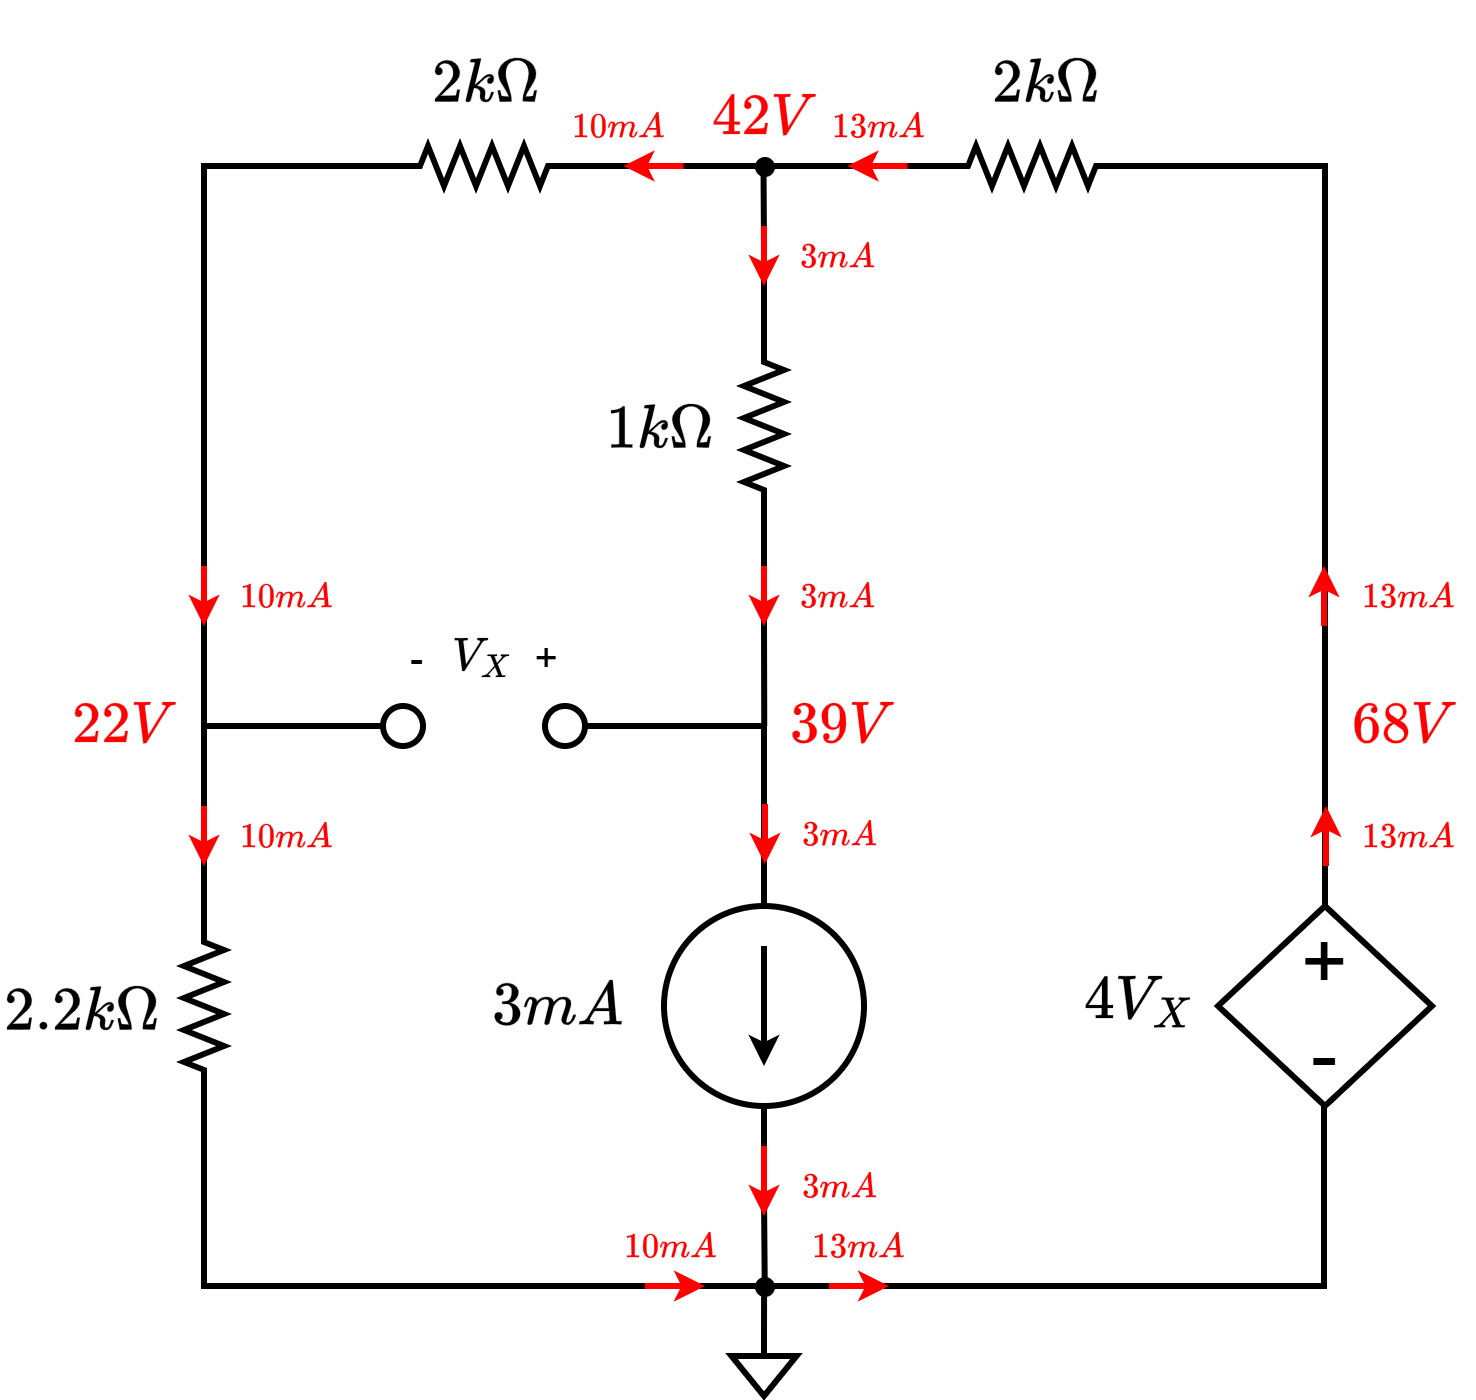
\includegraphics[width=0.5\textwidth]{questionbank/networks/wye_delta_nodal/v0/wye_kcl_sol.png}
\end{center}

Subbing in the voltages that we have already found, the problem proceeds just like part (\cref{prob:wye_delta_nodal:deltakcl}) for finding the current through the new resistors. Beautifully, the numbers are all familiar and the solution is undisturbed.

We show that KCL is satisfied for all the nodes again. Most nodes now only have two connections so they are quite simple.

At Common: \(13 -3-10  = 0\)

At Node 1: \(10 - 10 = 0\)

At Node 2: \(3-3=0\)

At Node 3: \(13 - 13 = 0\)

At Ground: \(10 + 3-13 = 0\)


Excellent. Consider for a moment how you might have solved the problem if you hadn’t used a Delta-Wye transform.
\end{answer}
\end{partquestion}

\end{mainquestion}